\documentclass[a4paper]{article}
\usepackage[utf8]{inputenc} % Skal passe til editorens indstillinger
\usepackage[english]{babel} % danske overskrifter


\newcommand{\name}{Carsten Nielsen}
%\newcommand{\stnumber}{s123369, s123161, s123821}
\newcommand{\course}{INI 404 Neuromorphic Engineering~I}
\newcommand{\university}{University of Zürich}
\newcommand{\studyline}{Institute of Neuroinformatics}
\newcommand{\assignment}{Lab 8 Post-Lab}
\renewcommand{\date}{\today} %If another date, than that of today is desiered


% Palatino for rm and math | Helvetica for ss | Courier for tt
\usepackage{mathpazo} % math & rm
\linespread{1.05}        % Palatino needs more leading (space between lines)
\usepackage{palatino} % tt
\normalfont
\usepackage[T1]{fontenc}
\usepackage[english]{babel}

\usepackage{graphicx}%allerese hentet % indsættelse af billeder
\usepackage{epstopdf} %Tilfj "--enable-write18" i argumentet for LaTex build. Dette vil konvertere .eps figurer til pdf-format
\graphicspath{{./picture/}} % stivej til bibliotek med figurer
\usepackage{subcaption} %Til gruppering af figurer
\usepackage{amsmath} %matpakke
\usepackage{amsfonts} %
\usepackage{amssymb} %
\usepackage{steinmetz} % flere matematik symboler
\usepackage{polynom} %for displaying polynom division
\usepackage{mathtools} % matematik - understøtter muligheden for at bruge \eqref{}
\usepackage{float}
\usepackage{placeins}
\usepackage{hhline}

%
\usepackage[usenames,dvipsnames]{xcolor}
\usepackage[compact,explicit]{titlesec}% http://ctan.org/pkg/titlesec
%
\usepackage[europeanresistors]{circuitikz}
\usepackage{pgfplots}
\usepgfplotslibrary{patchplots}
\pgfplotsset{compat=1.11}

%---------%
%Easy edit%
%---------%

%Section formating. arg1 is supplied when making section
\newcommand\presectionnumber[1]{~~}
\newcommand\postsectionnumber[1]{}
\newcommand\midlesection[1]{#1}
\newcommand\sectionnum[1]{\arabic{#1}}
\newcommand\subsectionnum[1]{\arabic{#1}}
\newcommand\subsubsectionnum[1]{\alph{#1}}



%------------%
%setion setup%
%------------%
\renewcommand\thesection{Opgave~\sectionnum{section}} %pas p�, kun i matematik
\renewcommand\thesubsection{\thesection,~\subsectionnum{subsection}}
\definecolor{MagRed}{RGB}{190,40,15}
\definecolor{MathGreen}{RGB}{82,164,0}

\titleformat{\section}{\normalfont\sffamily\large\bfseries\color{MathGreen}}{}{0pt}{|\kern-0.15ex|\kern-0.15ex|\kern-0.15ex|\presectionnumber{#1}\sectionnum{section}\postsectionnumber{#1}\qquad\quad\midlesection{#1}\label{sec:\sectionnum{section}}}
\titleformat{\subsection}[runin]{\large\bfseries}{}{10pt}{\sectionnum{section}.\subsectionnum{subsection})~#1\label{sec:\sectionnum{section}.\subsectionnum{subsection}}}
\titleformat{\subsubsection}[runin]{\itshape}{}{0pt}{\subsectionnum{subsection},\subsubsectionnum{subsection}~#1\label{sec:\sectionnum{section}.\subsectionnum{subsection}.\subsubsectionnum{subsubsection}}}
%\titleformat{\subsubsection}{\bfseries}{}{0pt}{\alph{subsection}.\arabic{subsubsection})\qquad\quad#1\label{\arabic{section}\alph{subsection}\arabic{subsubsection}}}

%----------%
%page setup%
%----------%
\textwidth = 400pt
\marginparwidth = 86pt
\hoffset = -25pt
\voffset= -30pt
\textheight = 670pt

%--------%
%hyperref%
%--------%
\newcommand{\HRule}{\rule{\linewidth}{0.5mm}}
\usepackage{fancyhdr}
\usepackage[plainpages=false,pdfpagelabels,pageanchor=false]{hyperref} % aktive links
\hypersetup{%
  pdfauthor={\name},
  pdftitle={\assignment},
  pdfsubject={\course} }
%\usepackage{memhfixc}% rettelser til hyperref

%-------------%
%Headder setup%
%-------------%
\fancyhf{} % tom header/footer
\fancyhfoffset{20pt}
\fancyhfoffset{20pt}
\fancyhead[OL]{\name \\ INI 404}
\fancyhead[OC]{Date \\ \date}
\fancyhead[OR]{\university\\ \studyline}
\fancyfoot[FL]{}
\fancyfoot[FC]{\thepage}
\fancyfoot[FR]{}
\renewcommand{\headrulewidth}{0.4pt}
\renewcommand{\footrulewidth}{0.4pt}
\headsep = 35pt
\pagestyle{fancy}
 % style setup

%Listings%
\usepackage{listingsutf8}
\usepackage[framed,numbered]{matlab-prettifier}


%setup listings
\lstset{language=Matlab,
  extendedchars=true,
  language=Octave,                % the language of the code
  basicstyle=\ttfamily\footnotesize,           % the size of the fonts that are
  % used for the code
  numbers=left,                   % where to put the line-numbers
  numberstyle=\tiny\color{gray},  % the style that is used for the line-numbers
  stepnumber=2,                   % the step between two line-numbers. If it's 1, each line 
                                  % will be numbered
  numbersep=5pt,                  % how far the line-numbers are from the code
  backgroundcolor=\color{white},      % choose the background color. You must add \usepackage{color}
  showspaces=false,               % show spaces adding particular underscores
  showstringspaces=false,         % underline spaces within strings
  showtabs=false,                 % show tabs within strings adding particular underscores
  frame=single,                   % adds a frame around the code
  rulecolor=\color{black},        % if not set, the frame-color may be changed on line-breaks within not-black text (e.g. comments (green here))
  tabsize=4,                      % sets default tabsize to 2 spaces
  captionpos=b,                   % sets the caption-position to bottom
  breaklines=true,                % sets automatic line breaking
  breakatwhitespace=false,        % sets if automatic breaks should only happen at whitespace
  title=\lstname,                   % show the filename of files included with \lstinputlisting;
                                  % also try caption instead of title
  %keywordstyle=\color{blue},          % keyword style
  %commentstyle=\color{dkgreen},       % comment style
  %stringstyle=\color{mauve},         % string literal style
  escapeinside={\%*}{*)},            % if you want to add LaTeX within your code
  morekeywords={*,...},              % if you want to add more keywords to the set
  deletekeywords={...}              % if you want to delete keywords from the given language
}
\lstset{literate=
  {á}{{\'a}}1 {é}{{\'e}}1 {í}{{\'i}}1 {ó}{{\'o}}1 {ú}{{\'u}}1
  {Á}{{\'A}}1 {É}{{\'E}}1 {Í}{{\'I}}1 {Ó}{{\'O}}1 {Ú}{{\'U}}1
  {à}{{\`a}}1 {è}{{\`e}}1 {ì}{{\`i}}1 {ò}{{\`o}}1 {ù}{{\`u}}1
  {À}{{\`A}}1 {È}{{\'E}}1 {Ì}{{\`I}}1 {Ò}{{\`O}}1 {Ù}{{\`U}}1
  {ä}{{\"a}}1 {ë}{{\"e}}1 {ï}{{\"i}}1 {ö}{{\"o}}1 {ü}{{\"u}}1
  {Ä}{{\"A}}1 {Ë}{{\"E}}1 {Ï}{{\"I}}1 {Ö}{{\"O}}1 {Ü}{{\"U}}1
  {â}{{\^a}}1 {ê}{{\^e}}1 {î}{{\^i}}1 {ô}{{\^o}}1 {û}{{\^u}}1
  {Â}{{\^A}}1 {Ê}{{\^E}}1 {Î}{{\^I}}1 {Ô}{{\^O}}1 {Û}{{\^U}}1
  {œ}{{\oe}}1 {Œ}{{\OE}}1 {æ}{{\ae}}1 {Æ}{{\AE}}1 {ß}{{\ss}}1
  {ç}{{\c c}}1 {Ç}{{\c C}}1 {ø}{{\o}}1 {å}{{\r a}}1 {Å}{{\r A}}1
  {€}{{\EUR}}1 {£}{{\pounds}}1
}

 \lstloadlanguages{% Check Dokumentation for further languages ...
         %[Visual]Basic
         %Pascal
         %C
         %C++
         %XML
         %HTML
         %Java
         %VHDL
         Matlab
 }
 %Listings slut%









%Matematik hurtige ting
%fed
\renewcommand\vec[1]{\mathbf{#1}}
\newcommand\matr[3]{{}_{#2}\mathbf{#1}{}_{#3}}
\newcommand\facit[1]{\underline{\underline{#1}}}
%\renewcommand\d[3]{\frac{\mbox{d}^{#3}#1(#2)}{\mbox{d}#2^{#3}}}
%underline
%\renewcommand\vec[1]{\underline{#1}}
%\newcommand\matr[3]{{}_{#2}\underline{\underline{#1}}{}_{#3}}

\renewcommand\matrix[4]{ %{alignment}{to space}{from space}{matrix}
{\vphantom{\left[\begin{array}{#1}#4\end{array}\right]}}_{#2}\kern-0.5ex
\left[\begin{array}{#1}
#4
\end{array}\right]_{#3}
}
\newcommand\e[0]{\mbox{e}}
\newcommand\E[1]{\cdot 10^{#1}}
\newcommand\im[0]{i}

\newcommand\Jaco{\mbox{Jacobi}}
\newcommand\del[2]{\frac{\partial {#1}}{\partial {#2}}}
\newcommand\abs[1]{\left| {#1} \right|}
\newcommand\stdfig[4]{ %width,img,cap,lab
\begin{figure}[H]
\centering
\includegraphics[width={#1}\textwidth]{#2}
\caption{#3}
\label{#4}
\end{figure}
}
\newcommand\stdfignoscale[3]{ %img,cap,lab
\begin{figure}[H]
\centering
\includegraphics{#1}
\caption{#2}
\label{#3}
\end{figure}
}
\newcommand\diff{\dot}
\newcommand\ddiff{\ddot}
\newcommand\dddiff{\dddot}
\newcommand\ddddiff{\ddddot}






% How to make ref to books or urls in bib
%\citetitle[fx: page 1]{name of ref in bib}


\tikzset{rrail/.style={rground,yscale=-1}}
\newcommand{\reffig}[1]{Fig.~\ref{#1}}

\begin{document}
\begin{titlepage}
\centering \parindent=0pt

\vspace*{\stretch{1}} \HRule\\[1cm]\Huge
\course\\[0.7cm]
\large \assignment\\[1cm]
\HRule\\[4cm]  
%\includegraphics[width=6cm]{picture}\\ Use this if you want a picture on the frontpage
\name\\
%\stnumber
TAs: Ning Quiao, Chenghan Li

\vspace*{\stretch{2}} \normalsize %

\begin{center}
	\date 
\end{center}
\vspace*{\stretch{2}} \normalsize
\begin{flushright}
%\includegraphics[width=6cm]{./dtu.eps}\\
\end{flushright}
\end{titlepage}

\newpage
\section{Experiment 1}

We measured the dependence of the differential pair currents \(I_1\) and \(I_2\) on the differential input voltage \(\delta V\). The results can be seen in \reffig{fig:ex1}. The linear fits have been done with the values of the currents for \(-0.04 \le V_1-V_2 \le 0.04\), where they present a stronger linearity. The equations for the fits are
\begin{align*}
&I_1  = 1.414\cdot10^{-7}(V_1-V_2 )+1.23\cdot10^{-8} \\
&I_2  = -1.406\cdot10^{-7}(V_1-V_2 )+1.18\cdot10^{-8} \\
&I_1+I_2  = 4\cdot10^{-10}(V_1-V_2 )-2.24\cdot10^{-8} \\
&I_1-I_2  = 2.821\cdot10^{-7}(V_1-V_2 )+5\cdot10^{-10}
\end{align*}

From these equations we calculate the offset voltage that makes \(I_1=I_2\) as \(-1.8 mV\). 

As shown in exercise 5b of the pre-lab, the slope of \(I_1-I_2\) is
\begin{equation*}
g_m = \frac{dI_{out}}{dV_{in}} = \frac{I_b\kappa}{2U_T}
\end{equation*}
%
Assuming that the currents change linearly between 0 and \(I_b\), we can approximate the voltage range in which the currents change linearly
\begin{equation*}
\Delta V_{linear} \cdot g_m = I_b
\end{equation*}
\begin{equation*}
\Delta V_{linear} = \frac{I_b}{g_m}=\frac{2U_T}{\kappa}
\end{equation*}
We can see that the linear range is proportional to the thermal voltage, \(U_T\).

\begin{figure}
    \center
    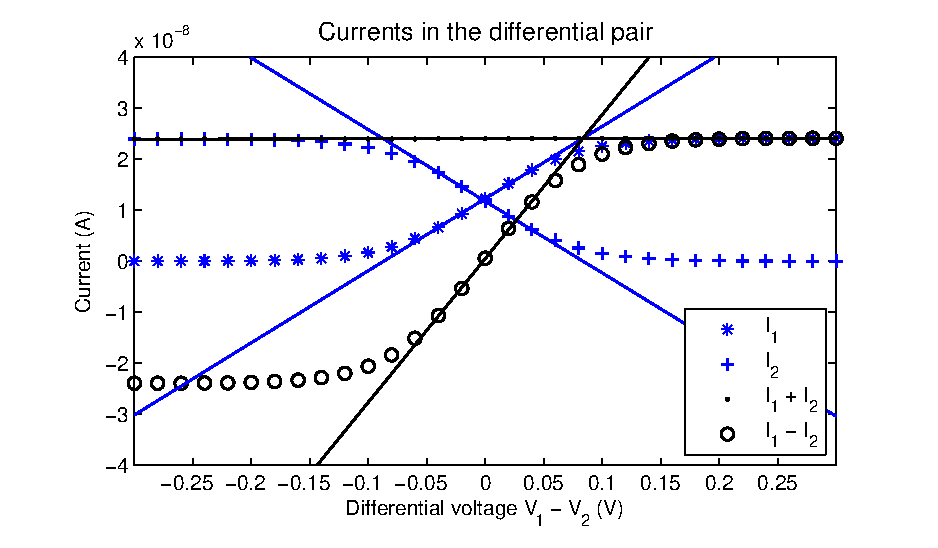
\includegraphics{q1.eps}
    \caption{Currents \(I_1\), \(I_2\), \(I_1+I_2\) and \(I_1-I_2\) in a differential pair as a function of the differential input voltage, \(V_1-V_2\), and their respectives linear fits for small input voltage.}
    \label{fig:ex1}
\end{figure}

If we run the differential pair in strong inversion, we find that the linear range is now proportional to \(V_b\)
\begin{equation*}
g_m = \frac{dI_{out}}{dV_{in}} = \sqrt{\beta I_b}
\end{equation*}
\begin{equation*}
\Delta V_{linear} = \frac{I_b}{g_m}=\sqrt{\frac{I_b}{\beta}} = \sqrt{\frac{k}{2}}(V_b-V_T)
\end{equation*}
\\
\section{Experiment 2}

We now measure the input-output relationship of the bump-antibump circuit. The experimental results can be seen in \reffig{fig:ex2}

\begin{figure}[!htb]
	\center
	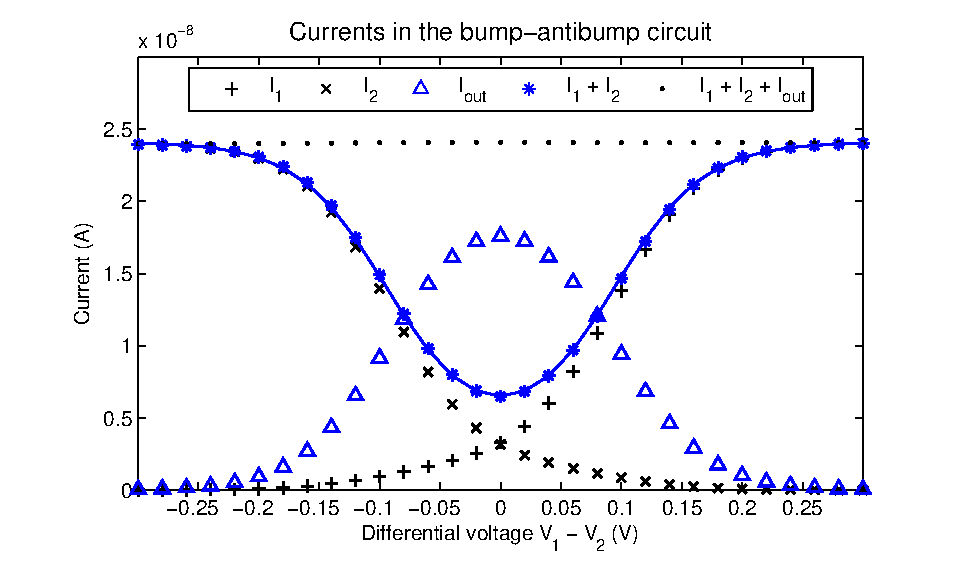
\includegraphics{q2.eps}
	\caption{Currents \(I_1\), \(I_2\), \(I_{out}\), \(I_1+I_2\) and \(I_1+I_2+I_{out}\) in a bump-antibump circuit as a function of the differential input voltage, \(V_1-V_2\). The line corresponds to a non-linear fit of the anti-bump current.}
	\label{fig:ex2}
\end{figure}

From question 4b of the prelab we know that 
\begin{equation*}
I_{anti-bump} = I_b-\frac{I_b}{1+\frac{4}{r}cosh^2(\frac{\kappa \Delta V}{2U_T})}
\end{equation*}
We did a non-linear fit to the experimental data using the model specified by this equation with parameters \(I_b, r, \kappa\) and \(U_T\) and got the following result, which is plotted in the Fig.2:

\begin{equation*}
I_{anti-bump} = 2.41\cdot10^{-8}-\frac{2.41\cdot10^{-8}}{1+\frac{4}{10.8}cosh^2(\frac{0.45 \Delta V}{2\cdot0.033})}
\end{equation*}

When \(V_1=V_2\), the current through the middle branch is given by

\begin{equation*}
I_{out} = \frac{I_b}{\frac{4}{r}+1}
\end{equation*}
where 
\begin{equation*}
r = \frac{\frac{W}{L}\big|_{out}}{\frac{W}{L}\big|_{in}} 
\end{equation*}
According to the specified widths and lengths of the transistors, \(r\) is supposed to be 5 . With this we obtain
\begin{equation*}
I_{out} = \frac{5}{9}I_b=0.56I_b
\end{equation*}
However, we find \(I_{out}\) to be \(0.73I_b\).
If we now use \(r=10.8\) as obtained from the non-linear fit, we get the correct value \(I_{out}=0.73I_b\). 

The discrepancy in the value of \(r\), which makes \(I_{out}\) larger than expected, can be caused by a short-channel effect. Because the transistors in the middle branch are shorter than those in the side branches and their \(Vds\) is large, they will be more affected by the Early effect and more current will flow through them.\\ 

\section{Experiment 3}
Here we measure the transconductance amplifier output current as a function of the input differential voltage for the circuit operating in subthreshold and above threshold. The results for the subthreshold case are shown in \reffig{fig:ex3a}. 
The equation of the linear fit for \(V_b=0.6\) and \(-0.06 \le V_1-V_2 \le 0.06\) is given by
\begin{equation*}
I_{out}= 1.014\cdot10^{-6}(V_1-V_2)+4.4\cdot10^{-9}
\end{equation*}

The slope of the fit should correspond to \(g_m=\frac{I_b\kappa}{2U_T}\) which is approximately \(g_m=\frac{0.9\cdot10^{-7}\cdot0.7}{2\cdot0.025}=1.3\cdot10^{-6}\).

\begin{figure}[!htb]
	\center
	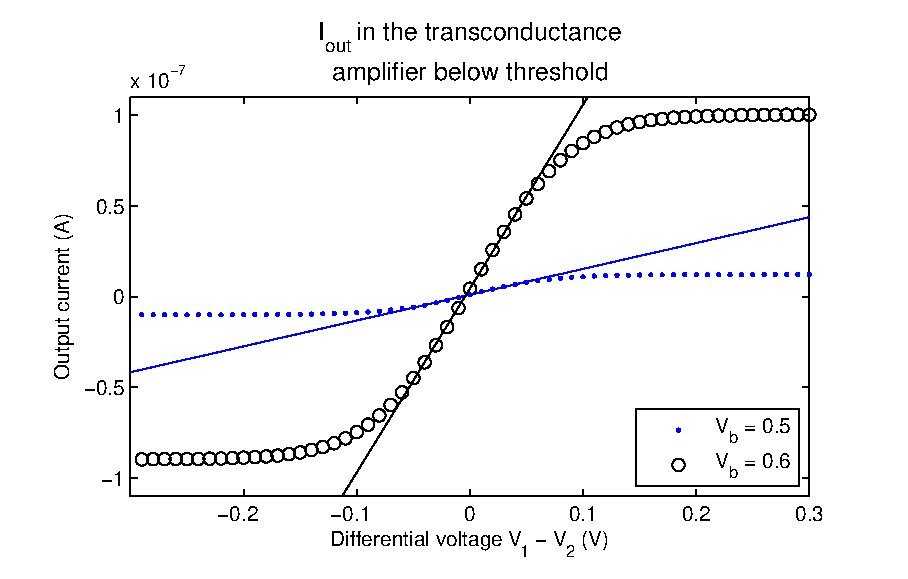
\includegraphics{q3a.eps}
	\caption{Output current, \(I_{out}\), as a function of the input voltage in a transconductance amplifier operating in sub-threshold for two values of \(V_b\) and linear fits for \(-0.06 \le V_1-V_2 \le 0.06\).}
	\label{fig:ex3a}
\end{figure}

We can observe that \(|I_{out}|\) is larger for \(V_1\gg V_2\) than for \(V_2\gg V_1\) although ideally they should be identical in both cases and equal to \(I_b\). When \(V_2\gg V_1\), \(M_1\) should be cutt off and \(M_2\) should conduct \(I_b\), therefore, the saturation value of the current in this case should indeed be \(-I_b\). From this we deduce that it is the value of the current for \(V_1\gg V_2\) which is larger than expected. This would be explained by the current mirror having  a gain larger than one due to a mismatch in the transistor sizes. 

From the plot we also can observe that there is an offset in the input voltage. This can be caused by different non-idealities. One of them is the one just mentioned above; since the current mirror is making a larger copy, in order to have \(I_{out}=0\) we need to have \(V_1<V_2\). Another way of saying this is that when \(V_1=V_2\), we will have a positive value of \(I_{out}\) which is what we get from the linear fit. 

Another non-ideality that can cause an offset voltage is a mismatch between the transistors of the differential pair. Finally this also can be due to the Early effect and the fact that \(V_{ds}\) is different for both transistors of the pair. 

These last two phenomena will cause an offset voltage but not a difference in the saturation values of \(|I_{out}|\) which allows us to distinguish wether the problem is located in the differential pair or in the current mirror. 


\begin{figure}[!htb]
	\center
	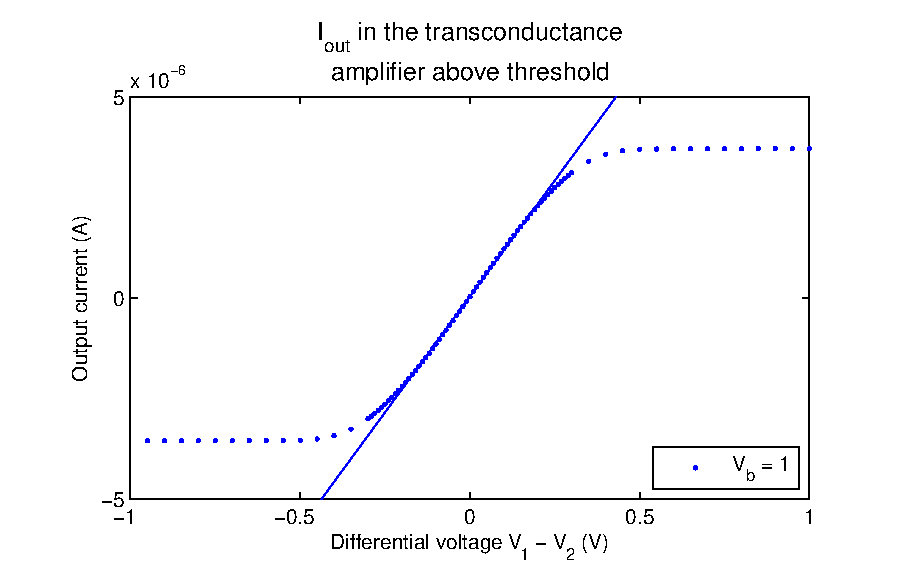
\includegraphics{q3b.eps}
	\caption{Output current, \(I_{out}\), as a function of the input voltage in a transconductance amplifier operating above threshold and a linear fit for \(-0.06 \le V_1-V_2 \le 0.06\).}
	\label{fig:ex3b}
\end{figure}


\section{Experiment 4}

We measured the open-circuit volgate gain of the amplifier. The results are shown in Fig. 5. We obtained a gain of \(626\) in the high-gain region as can be seen in the equation for the fit
\begin{equation*}
V_{out}=626.13(V_1-V_2)+0.75
\end{equation*}

\begin{figure}[!htb]
	\center
	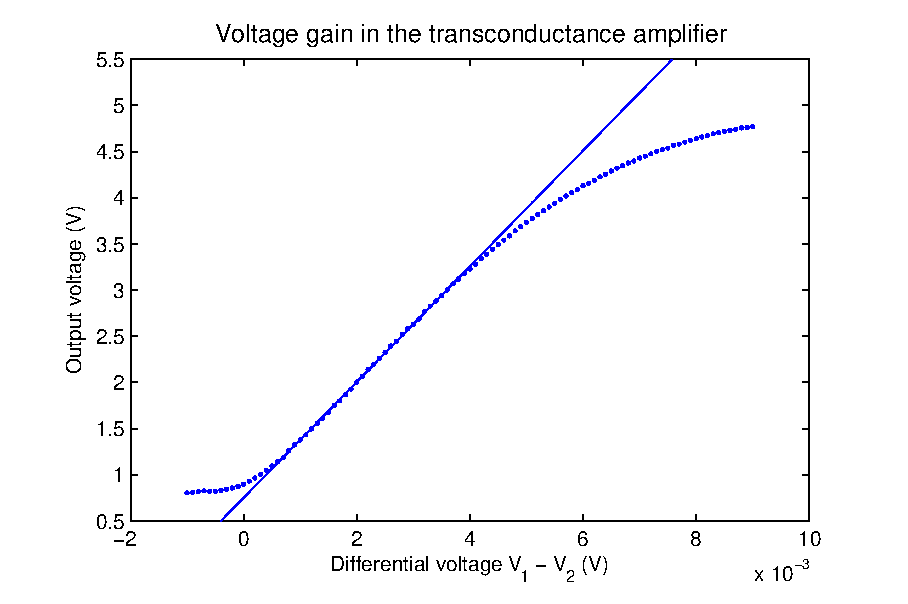
\includegraphics{q4a.eps}
	\caption{Output voltage, \(V_{out}\), as a function of the input voltage in a transconductance amplifier operating in open circuit and in subthreshold. The line corresponds to a linear fit in the high-gain region.}
	\label{fig:ex4a}
\end{figure}

\begin{figure}[!htb]
	\center
	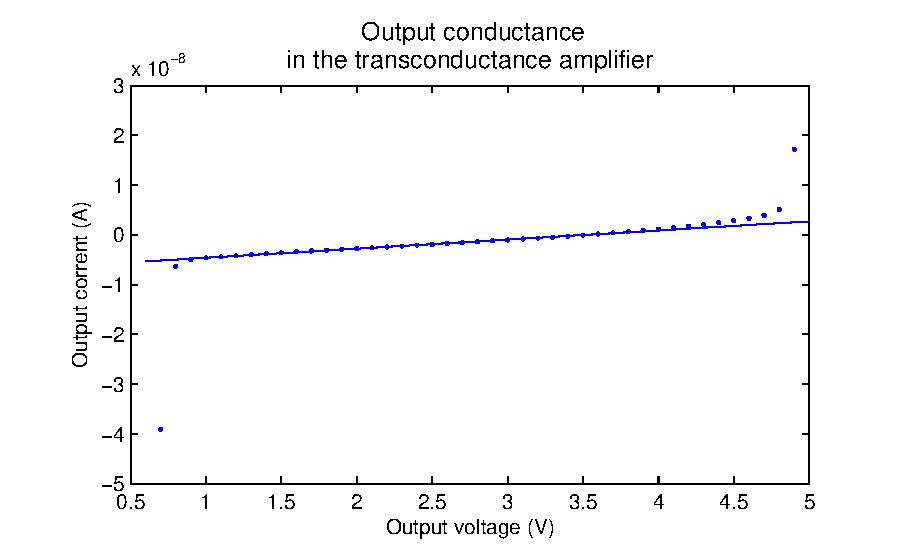
\includegraphics{q4b.eps}
	\caption{Output current, \(I_{out}\), as a function of the output voltage in a transconductance amplifier operating in subthreshold and a fit in the linear region.} .
	\label{fig:ex4b}
\end{figure}

We then measured the output current of the amplifier as a function of the output voltage to calculate the output conductance. The experimental results can be seen in Fig 6. and the equation for the fit is given by
\begin{equation*}
I_{out}=1.829\cdot10^{-9}V_{out}-6.429\cdot10-^{9}
\end{equation*}
The output conductance is the slope of the fit, \(g_d = 1.829\cdot10^{-9}\). 

With this value of \(g_d\) and the value of \(g_m\) calculated in experiment 3,  we can estimate the voltage gain as \(A=\frac{g_m}{g_d}\) and compare it with the measured one. 
\begin{equation*}
A=\frac{g_m}{g_d}=\frac{1.014\cdot10^{-6}}{1.829\cdot10^{-9}}=554.3
\end{equation*}

This estimated voltage gain presents a \(11.5\%\) error.
\begin{equation*}
e=\frac{554.3-626.1}{626.1}\cdot100=11.46\%
\end{equation*}

Finally, we measured the voltage gain of the wide-range transconductance amplifier. The results are shown in \reffig{fig:ex4c} and the equation for the fit is
\begin{equation*}
V_{out}=3996.6(V_1-V_2)-28.69
\end{equation*}
Compared to the 5-transistors amplifier, we observe a wider range in which there is linear amplification and a higher gain. The difference in the gain is due to the output transistors having \(W/L=3/58\) instead of \(6/6\). The longer the transistors, the smaller the Early effect and thus the higher the gain. 

\begin{figure}
	\center
	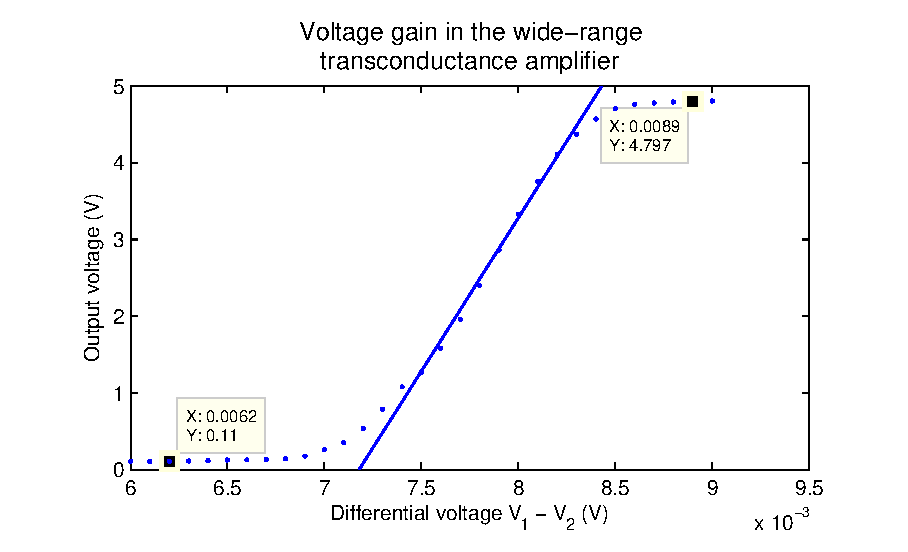
\includegraphics{q4c.eps}
	\caption{Output voltage as a function of the input voltage in the wide-range transconductance amplifier and a fit in the linear region.} .
	\label{fig:ex4c}
\end{figure}

\end{document}
